
%(BEGIN_QUESTION)
% Copyright 2009, Tony R. Kuphaldt, released under the Creative Commons Attribution License (v 1.0)
% This means you may do almost anything with this work of mine, so long as you give me proper credit

Read and outline the ``Characterized Valve Trim'' subsection of the ``Control Valve Characterization'' section of the ``Control Valves'' chapter in your {\it Lessons In Industrial Instrumentation} textbook.  Note the page numbers where important illustrations, photographs, equations, tables, and other relevant details are found.  Prepare to thoughtfully discuss with your instructor and classmates the concepts and examples explored in this reading.

\underbar{file i04238}
%(END_QUESTION)





%(BEGIN_ANSWER)


%(END_ANSWER)





%(BEGIN_NOTES)

Since the fundamental problem of varying differential pressure at the valve cannot be avoided in most applications, we must find some other way to make a control valve's behavior more linear.  One way is to intentionally design the valve trim so that it opens ``slowly'' at small stem positions and more aggressively at large stem positions.  In other words, we build the valve so that it is nonlinear in its own way, that complements the nonlinearity of the process's load line.

\vskip 10pt

A valve whose $C_v$ varies linearly with stem travel has a {\it linear} inherent characteristic.  A valve built to exhibit rapid increases in $C_v$ as soon as the plug lifts off the seat has a {\it quick-opening} inherent characteristic.  A valve designed to be nonlinear in a manner complementary to drooping pressure has an {\it equal-percentage} inherent characteristic.

$$\includegraphics[width=15.5cm]{i04238x01.eps}$$

$$C_v = x C_{vm} \hskip 30pt \hbox{\bf Linear trim}$$

$$C_v = C_{vm} R^{(x - 1)}  \hskip 30pt \hbox{\bf Equal percentage trim}$$

Different characteristics are implemented in valve bodies by shaping the valve trim in different ways (different shapes of plugs, of ports, of cages, or of balls).  One may also program a valve positioner to implement different characterizations, by moving the valve stem in a manner that is not directly proportional to the command signal.






\vskip 20pt \vbox{\hrule \hbox{\strut \vrule{} {\bf Suggestions for Socratic discussion} \vrule} \hrule}

\begin{itemize}
\item{} Explain how valve characterization helps to overcome the problem of ``process distortion'' seen when differential pressure across the valve decreases with increased flow.
\item{} What must one do to alter the characteristic of a control valve once it's been purchased?
\item{} Examine the illustrations of differently-shaped valve trim components, and explain how each shape yields the desired opening characteristic.
\end{itemize}

%INDEX% Reading assignment: Lessons In Industrial Instrumentation, control valve characterization (characterized trim)

%(END_NOTES)


